\let\negmedspace\undefined
\let\negthickspace\undefined
\documentclass[journal,12pt,twocolumn]{IEEEtran}
\usepackage{cite}
\usepackage{amsmath,amssymb,amsfonts,amsthm}
\usepackage{algorithmic}
\usepackage{graphicx}
\usepackage{textcomp}
\usepackage{xcolor}
\usepackage[justification=centering]{caption}
\usepackage{txfonts}
\usepackage{listings}
\usepackage{enumitem}
\usepackage{mathtools}
\usepackage{gensymb}
\usepackage{comment}
\usepackage[breaklinks=true]{hyperref}
\usepackage{tkz-euclide} 
\usepackage{listings}
\usepackage{gvv}                                        
\def\inputGnumericTable{}                                 
\usepackage[latin1]{inputenc}                                
\usepackage{color}                                            
\usepackage{array}                                            
\usepackage{longtable}                                       
\usepackage{calc}                                             
\usepackage{multirow}                                         
\usepackage{hhline}                                           
\usepackage{ifthen}                                           
\usepackage{lscape}

\newtheorem{theorem}{Theorem}[section]
\newtheorem{problem}{Problem}
\newtheorem{proposition}{Proposition}[section]
\newtheorem{lemma}{Lemma}[section]
\newtheorem{corollary}[theorem]{Corollary}
\newtheorem{example}{Example}[section]
\newtheorem{definition}[problem]{Definition}
\newcommand{\BEQA}{\begin{eqnarray}}
\newcommand{\EEQA}{\end{eqnarray}}
\newcommand{\define}{\stackrel{\triangle}{=}}
\theoremstyle{remark}
\newtheorem{rem}{Remark}
\begin{document}

\bibliographystyle{IEEEtran}
\vspace{3cm}

\title{10.5.4-5}
\author{EE23BTECH11033-killana jaswanth}
\maketitle
\newpage

\bigskip

\renewcommand{\thefigure}{\theenumi}
\renewcommand{\thetable}{\theenumi}
\textbf{Question}:\\
A small terrace at a football ground comprises of 15 steps each of which is 50
m long and built of solid concrete.Each step has a rise of 1/4 m and a tread of
1/2 m. Calculate the total volume of concrete required to build the terrace.
[Hint: Volume of concrete required to build the first step=\begin{align}
    \text{{volume}}=1/4 \cdot 1/2 \cdot 50 
\end{align}
\textbf{solution} 
\\\\\begin{tabular}{|c|c|}
\hline
\textbf{parameter for step one }& \textbf{value}
\\\hline
\multirow{3}{1em}\\length&50
\\breadth&$0.25$
\\height&$0.5$
\\volume&$6.25$ 
\\\hline
\end{tabular}
\\
\\=The height difference between any 2 consecutive steps is 0.25 m.
\\=So, the volume of the second step is (50m)(5m)(0.5m)= 12.5$m^3$ and third is 18.75$m^3$
\begin{align}
S_n = \frac{n+1}{2} [2a+(n)d]   
\\n=0,1,2,3,...
\end{align}
here\\
\\\begin{tabular}{|c|c|c|}
\hline
\textbf{parameter}& \textbf{value}& \textbf{measurement}
\\\hline
\multirow{3}{1em}\\a&$6.25$&first term
\\d&$6.25$&common diffrence
\\n&$14$&no of terms from 0
\\\hline
\end{tabular}
\begin{align}\\S_n &= \frac{14+1}{2} [12.5+(14)6.25]
\end{align}
\begin{align}
S_n = \frac{15}{2}[12.5(14)6.25]
\end{align}
   \begin{align}
   S_n = \frac{15}{2} [12.5+87.5]
   \end{align}
   \begin{align}
   volume=(7.5) \cdot 100
   &=750m^3
   \end{align}
\\\\\textbf{plot of x(n) and n}
\\\begin{align}
    \text{{x(n)}}=(a+n \cdot d ) \cdot u(n)
\end{align}
\begin{figure}[h]
    \renewcommand\thefigure{1}
    \centering
    \captionsetup{justification=centering}
    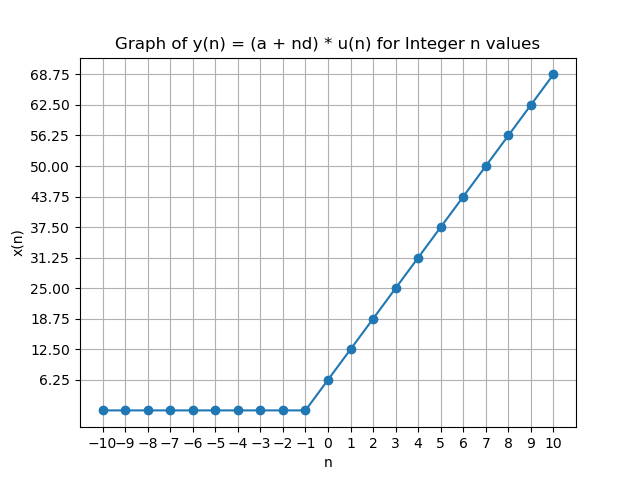
\includegraphics[width=1\linewidth]{Figure_1.png}
    \caption{}
    \label{stemplot2}
\end{figure}\begin{align}
\\x(n)\overset{Z}{\longleftrightarrow}  X(Z)
\\x(n)=(a+nd)u(n)
\\X(Z)&=\sum_{-\infty}^{\infty}x(n)Z^{-n}\
\\&=\sum_{-\infty}^{\infty}(a+nd)u(n)Z^{-n}\
\\&=0+\sum_{0}^{\infty}(a+nd)Z^{-n}\
\\&=\frac{x(0)}{1-\,z^{-1}}+\frac{dz^{-1}}{({1-{z^{-1}}})^2}\:\:,|z|>|r|
\\&=\frac{6.25}{1-\,z^{-1}}+\frac{6.25z^{-1}}{({1-{z^{-1}}})^2}\:\:,|z|>|r|
\end{align}
 \end{document}
